\documentclass[12pt]{extarticle}
%Some packages I commonly use.
\usepackage[portuguese]{babel}
\usepackage{graphicx}
\usepackage{framed}
\usepackage[normalem]{ulem}
\usepackage{amsmath}
\usepackage{amsthm}
\usepackage{amssymb}
\usepackage{amsfonts}
\usepackage{enumerate}
\usepackage[utf8]{inputenc}
\usepackage{float}
\usepackage{gensymb}
\usepackage[top=1 in,bottom=1in, left=1 in, right=1 in]{geometry}
\usepackage{multirow}
\usepackage{caption}
\usepackage{subcaption}
\usepackage[utf8]{inputenc}

%A bunch of definitions that make my life easier
\newcommand{\matlab}{{\sc Matlab} }
\newcommand{\cvec}[1]{{\mathbf #1}}
\newcommand{\rvec}[1]{\vec{\mathbf #1}}
\newcommand{\ihat}{\hat{\textbf{\i}}}
\newcommand{\jhat}{\hat{\textbf{\j}}}
\newcommand{\khat}{\hat{\textbf{k}}}
\newcommand{\minor}{{\rm minor}}
\newcommand{\trace}{{\rm trace}}
\newcommand{\spn}{{\rm Span}}
\newcommand{\rem}{{\rm rem}}
\newcommand{\ran}{{\rm range}}
\newcommand{\range}{{\rm range}}
\newcommand{\mdiv}{{\rm div}}
\newcommand{\proj}{{\rm proj}}
\newcommand{\R}{\mathbb{R}}
\newcommand{\N}{\mathbb{N}}
\newcommand{\Q}{\mathbb{Q}}
\newcommand{\Z}{\mathbb{Z}}
\newcommand{\<}{\langle}
\newcommand{\grad}{$^\circ$}
\renewcommand{\>}{\rangle}
\renewcommand{\emptyset}{\varnothing}
\newcommand{\attn}[1]{\textbf{#1}}
\theoremstyle{definition}
\newtheorem{theorem}{Theorem}
\newtheorem{corollary}{Corollary}
\newtheorem*{definition}{Definition}
\newtheorem*{example}{Example}
\newtheorem*{note}{Note}
\newtheorem{exercise}{Exercise}
\newcommand{\bproof}{\bigskip {\bf Proof. }}
\newcommand{\eproof}{\hfill\qedsymbol}
\newcommand{\Disp}{\displaystyle}
\newcommand{\qe}{\hfill\(\bigtriangledown\)}
\setlength{\columnseprule}{1 pt}
\usepackage[utf8]{inputenc}

\title{Aula 2 - Dilatação Térmica}
\author{Felipe Salvador}
\date{Atualizado em \today}

\begin{document}

\maketitle

\section{O que é dilatação térmica?}

Na aula passada, vimos que a temperatura é uma medida e noção de quão agitada e vibrante estão as moléculas de um objeto, líquido ou gás. Quanto maior essa agitação, vimos que maior é a temperatura. Muito bem, acontece que, conforme a temperatura dos objetos cresce, o espaço entre as moléculas começa a crescer, pelo fato de elas estarem se movimentando mais. 

Com isso, se eu olhar esse comportamento do espaçamento entre as moléculas de forma coletiva, eu começo a perceber que os meus objetos (objetos, líquidos e gases) começam a se expandir, crescer. O nome desse efeito é \textbf{Dilatação Térmica}.

Tudo isso que eu coloquei acima vale para quando diminuímos a temperatura. Quanto mais frio estiver um objeto, as moléculas estarão menos agitadas e, logo, menos espaço elas ocupam. Então, quando olho para o corpo, percebo que o corpo começa a diminuir e ficar menor.


Só que esse crescimento/decrescimento depende de corpo para corpo, de material para material, podendo ser muito pequeno, tal que podemos desprezar, ou podendo ser até grande.

Isso é uma das razões de a gente sentir uns trancos quando estamos num carro passando por uma ponte. Na ponte, os engenheiros não podem construir algo inteiro, sem partir a ponte em pedaços, porque o concreto, usado para construir a ponte, dilata e contraem bastante durante o dia por causa do aquecimento do Sol. Eles deixam uns vãos em certos lugares da ponte para que o concreto possa dilatar e contrair. Caso não fosse deixado esses vãos, o concreto iria quebrar e abrir rachaduras, o que é muito perigoso.

\begin{figure}[H]
    \centering
    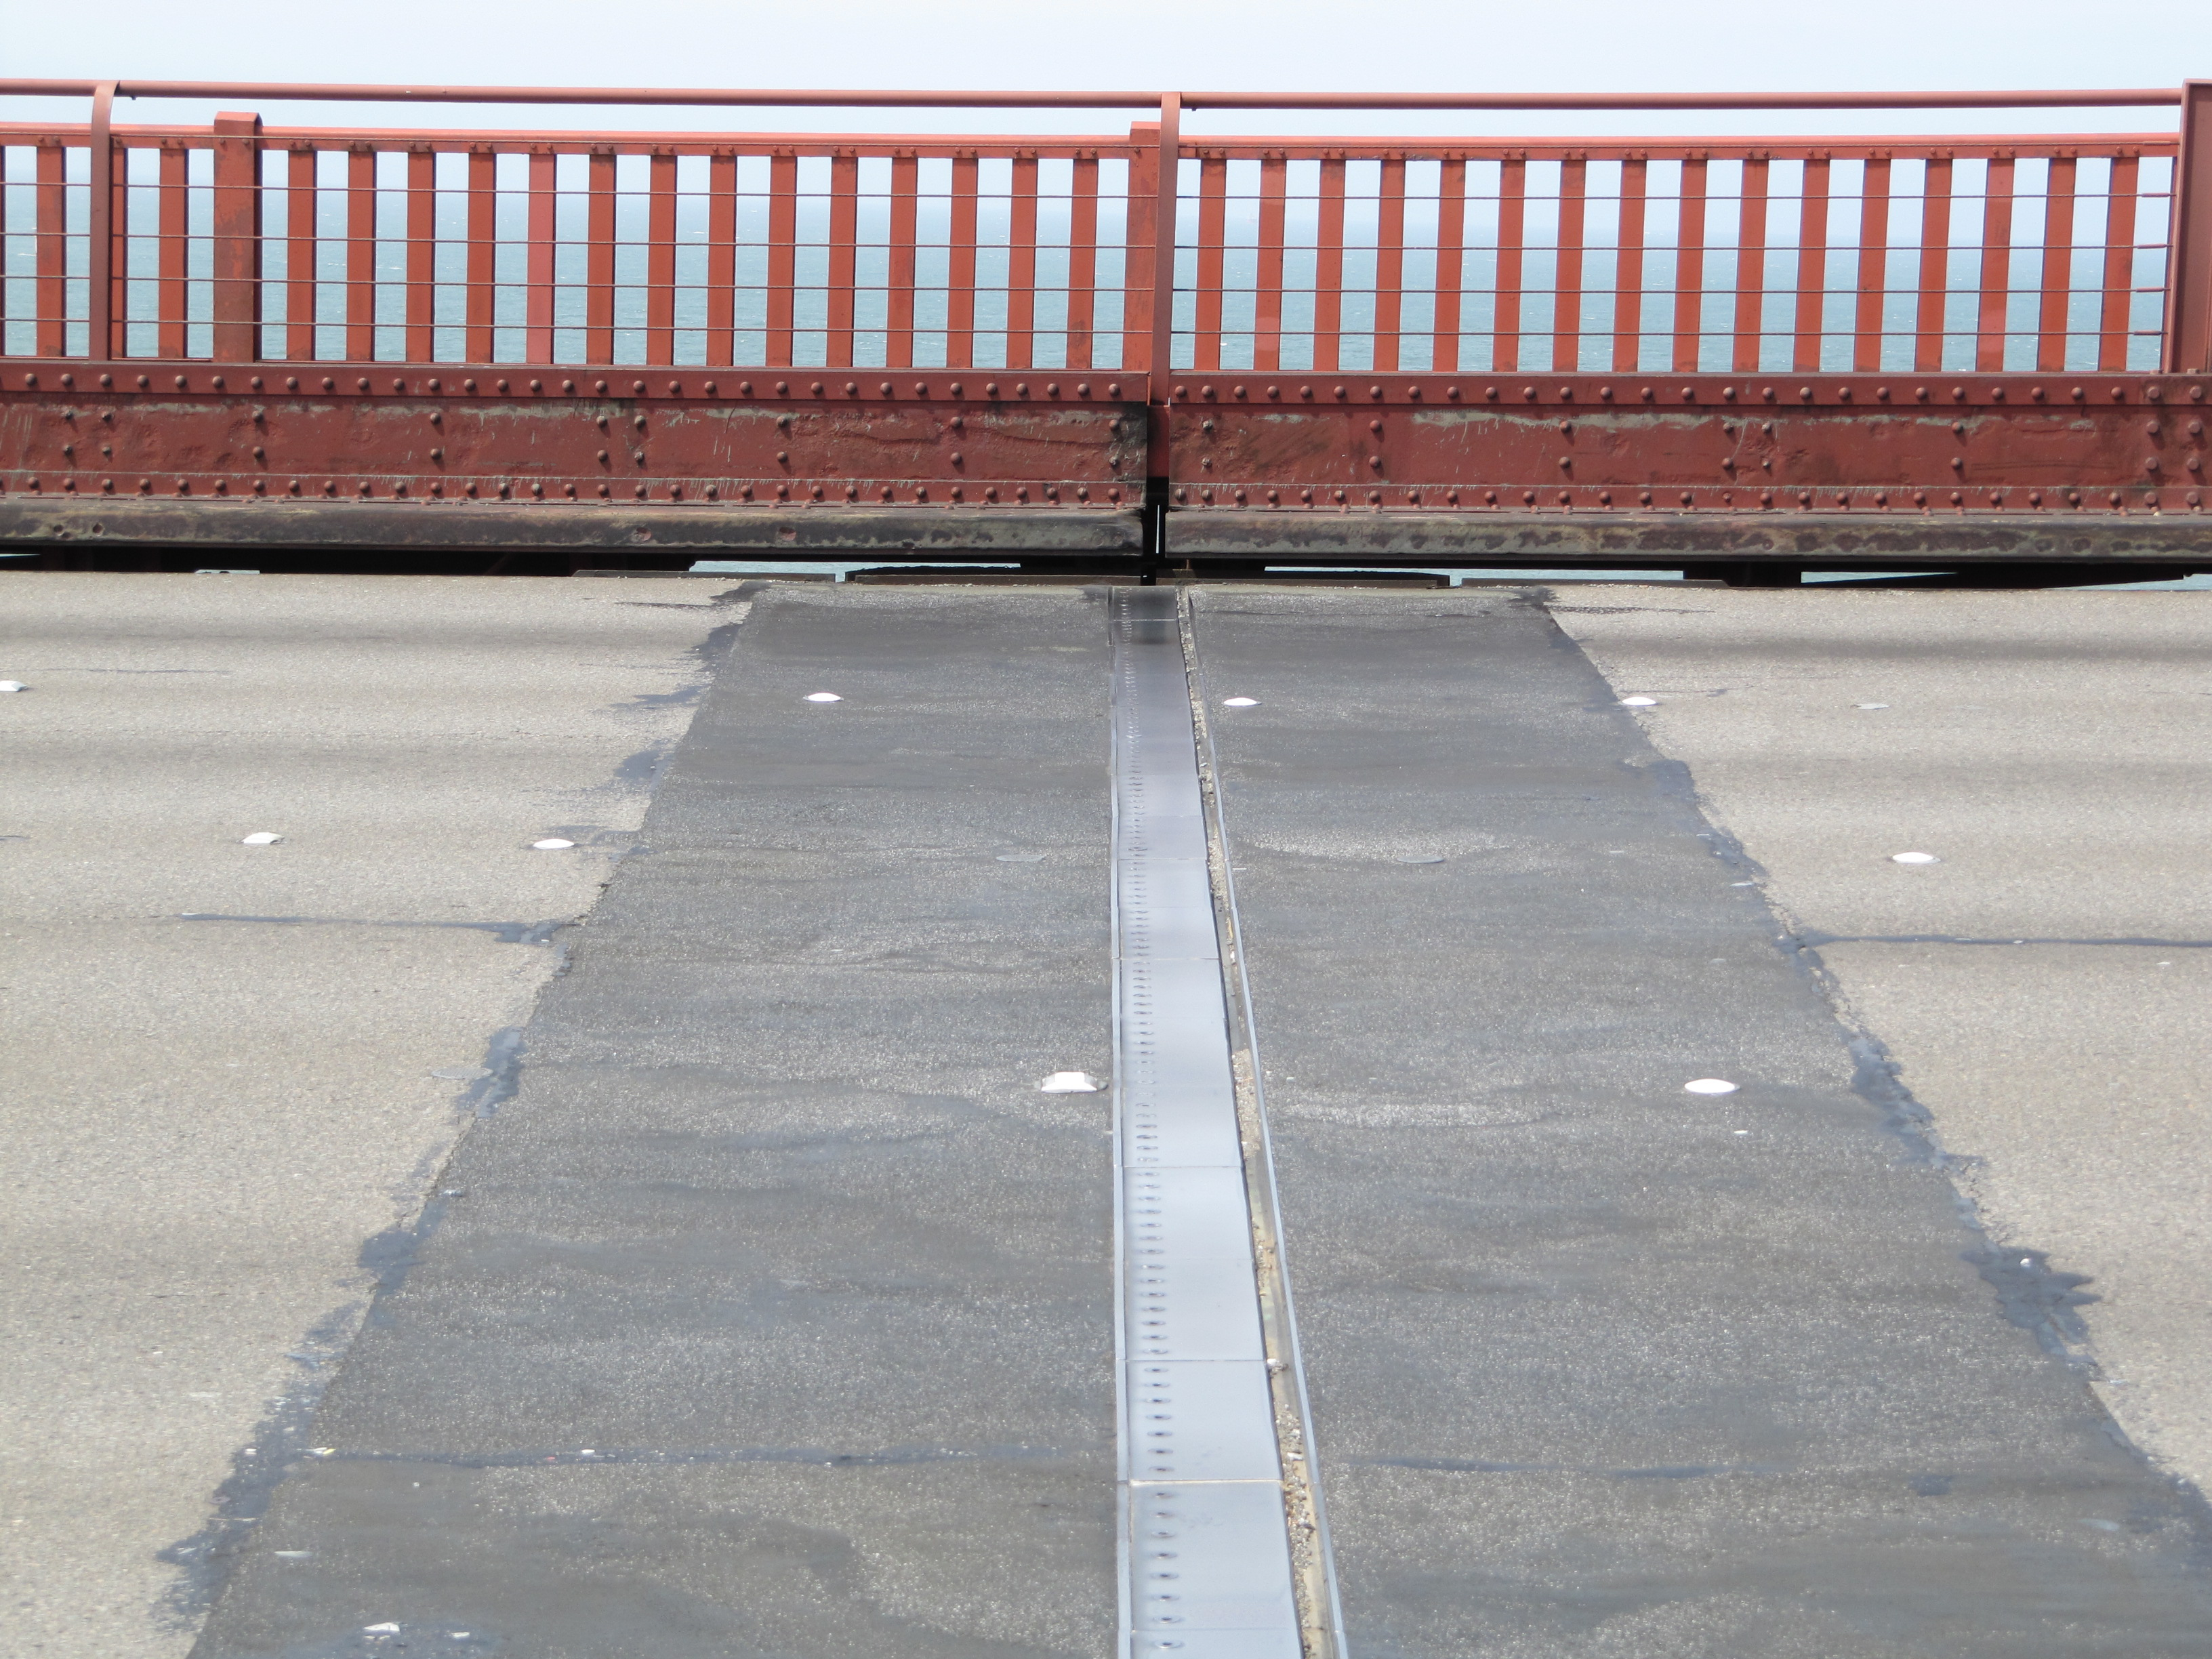
\includegraphics[width=0.7\textwidth]{Expansion_joint_Golden_Gate_Bridge.jpg}
    \caption{Foto de uma \textit{junta de dilatação} da Golden Gate em São Francisco nos EUA - esse é o nome desses vãos deixados numa ponte}
    \label{fig:ex_1}
\end{figure}

Além de pontes, juntas de dilatação são usadas em pisos que ficam expostos ao ambiente. Nesse caso, eles usam uma massinha bem elástica para absorver essa dilatação, assim não deixando 'buracos' nos pisos.

\begin{figure}[H]
    \centering
    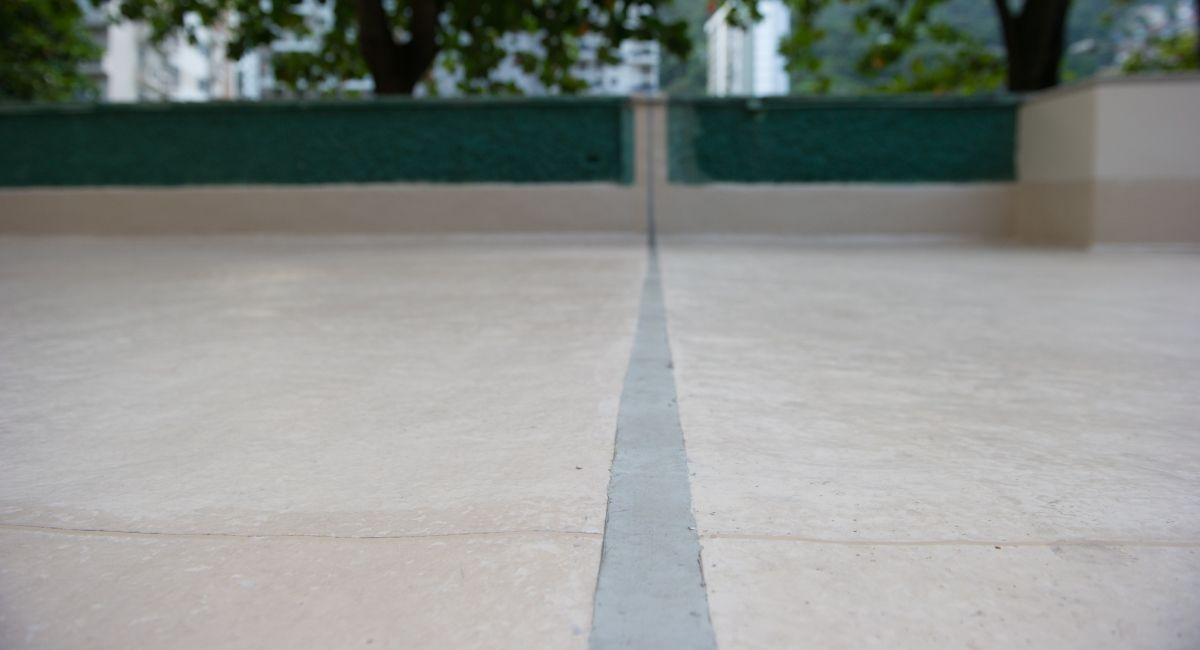
\includegraphics[width=0.7\textwidth]{xjuntas-de-dilatacao.jpg.pagespeed.ic.2LQSZrGsDX.jpg}
    \caption{Foto de uma junto de dilatação de um piso}
    \label{fig:ex_2}
\end{figure}

\section{Tipos de Dilatação}

Ao todo, vamos falar dos 3 tipos de dilatação que temos: Dilatação Linear (1 dimensão), Dilatação Superficial (2 dimensões) e Dilatação Volumétrica (3 dimensões).

\subsection{Dilatação linear}

Para objetos que são parecidos como uma barra, a dilatação linear acontece aumentando ou diminuindo o comprimento da barra, por exemplo. Existe uma fórmula que nos permite calcular o quanto uma barra cresce ou diminuiu e é dada por:
\begin{equation}
    \Delta L = L_0\, \alpha\, \Delta T
\end{equation}
\noindent em que $\Delta L$ é o quanto uma barra cresceu ou diminuiu e é dada por: $\Delta L = L - L_0$ ($L$ é o comprimento final da barra e $L_0$ é comprimento inicial dela), $\alpha$ é o \textbf{coeficiente de dilatação linear} e $\Delta T$ é a variação de temperatura que a barra sofreu.

Um detalhe importante: $\alpha$ depende do material de que a barra é feita, então, normalmente, é um valor dado no enunciado ou é pedido como exercício. 

Pela fórmula, a unidade do coeficiente de dilatação linear é:

\begin{equation}
    \begin{split}
        &\Delta L = L_0\, \alpha\, \Delta T\\
        &[L] = [L]*[\alpha]*[T] \\
        & 1 =[\alpha]*[T] \implies [\alpha] = \frac{1}{[T]} = [T]^{-1}
    \end{split}
\end{equation}
\noindent [L] é a unidade de comprimento, [T] é a unidade de temperatura. Ou seja, se a temperatura for dada em \grad C, então a unidade $\alpha$ é \grad C$^{-1}$

\begin{figure}[H]
    \centering
    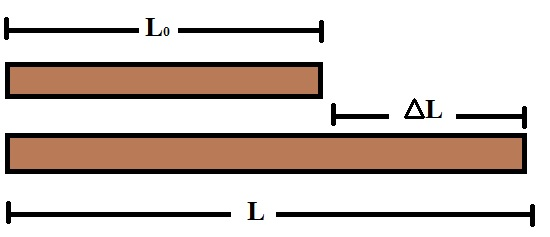
\includegraphics[width=0.5\textwidth]{dilatação linear de uma barra.jpg}
    \caption{Esquema da dilatação linear de uma barra}
    \label{fig:dilatacao_lin}
\end{figure}

\subsection{Dilatação Superficial}

Para placas, folhas, a dilatação ocorre aumentando ou diminuindo a área dessa folha/placa. A fórmula para a dilatação superficial é bem parecida com a da dilatação linear e é dada por:

\begin{equation}
    \Delta A = A_0\,\beta\, \Delta T
\end{equation}
\noindent em que $\Delta A$ é o quanto a área cresce ou diminui $\Delta A = A - A_0$, tal que $A$ é a área final da placa e $A_0$ é a área inicial, $\beta$ é o \textbf{coeficiente de dilatação superficial} e $\Delta T$ a variação da temperatura que a placa sofreu.

Fazendo a mesma análise de unidades, a unidade de $\beta$ é:

\begin{equation}
    \begin{split}
        &\Delta A = A_0\, \beta\,\Delta T\\
        &[A] = [A]*[\beta]*[T]\\
        &1 = [\beta]*[T] \implies [\beta] = \frac{1}{[T]} = [T]^{-1}
    \end{split}
\end{equation}
\noindent em que [A] é a unidade de área e [T] é a unidade de temperatura. Ou seja, a unidade de $\beta$ é igual à unidade de $\alpha$ da dilatação linear.

\begin{figure}[H]
    \centering
    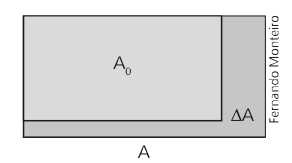
\includegraphics[width=0.5\textwidth]{dilatacao_superficial.png}
    \caption{Esquema de como a dilatação superficial funciona}
    \label{fig:dilatacao superficial}
\end{figure}

\textbf{Obs: caso a placa tenha um buraco, quando o corpo dilata, o buraco também aumenta e quando o corpo diminui, o buraco também diminui. O aumento/diminuição do buraco é dado pela mesma fórmula da dilatação superficial.}

\begin{figure}[H]
    \centering
    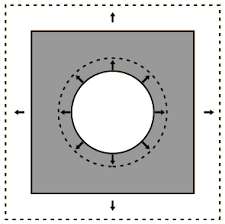
\includegraphics[width=0.4\textwidth]{download.png}
    \caption{Esquema da dilatação de uma placa com buraco. O buraco também aumenta conforme a placa dilata.}
    \label{fig:hole}
\end{figure}

\subsection{Dilatação volumétrica}

Por último, temos a dilatação volumétrica. Acontece em corpos cujas dimensões (altura, profundidade e largura) são importantes. Essa dilatação faz com que o volume desse corpo aumente ou diminua conforme a temperatura cresça ou caia. Novamente, a fórmula para essa dilatação é bem parecida com as outras:

\begin{equation}
    \Delta V = V_0\,\gamma\,\Delta T
\end{equation}
\noindent em que $\Delta V$ é quanto o volume aumentou ou diminui e é dado por $\Delta V = V - V_0$ ($V$ é o volume após a dilatação e $V_0$ é o volume antes dela), $\gamma$ (leia-se \textit{'gama'}) é o \textbf{coeficiente de dilatação volumétrica} e $\Delta T$ é a variação de temperatura.

Da mesma forma, a análise da dimensão/unidade de $\gamma$ é:

\begin{equation}
    \begin{split}
        &[V] = [V]*[\gamma]*[T]\\
        &1 = [\gamma]*[T] \implies \gamma= \frac{1}{[T]} = [T]^{-1}
    \end{split}
\end{equation}

\noindent em que [V] é a unidade de volume e [T] a de temperatura. Perceba que a unidade de $\gamma$ é igual à de $\beta$ e $\alpha$: $[T]^{-1}$, como por exemplo: $\gamma =\, ^\circ C^{-1}$

\textbf{Obs: caso o corpo tenha um buraco, quando o corpo dilata, o buraco também aumenta e quando o corpo diminui, o buraco também diminui. O aumento ou diminuição do volume do buraco também é dado pela fórmula de dilatação volumétrica.}

\begin{figure}[H]
    \centering
    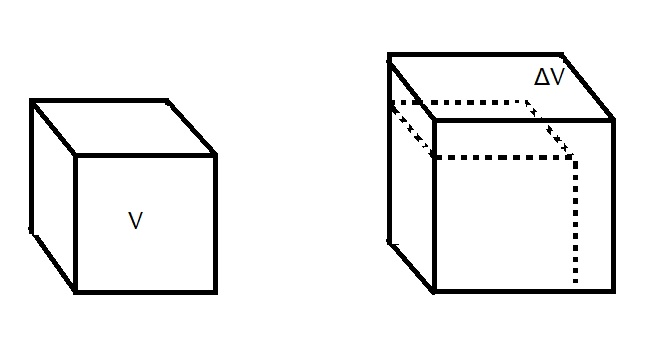
\includegraphics[width=0.5\textwidth]{aaed6390a9a14e9897c7dc8056a1ceff-xd5g0w (1).jpg}
    \caption{Esquema de como é a dilatação volumétrica}
    \label{fig:dilatacao_vol}
\end{figure}

\section{Relações entre os coeficientes de dilatação}

Como vimos, todos os coeficientes possuem a mesma unidade e a relação entre eles não para por ai. Podemos relacionar $\beta$ e $\gamma$ com o $\alpha$ por meio das seguintes igualdades:

\begin{equation}
    \boxed{\beta = 2\alpha;\quad\quad \gamma = 3\alpha}
\end{equation}

\section{Exemplos}

\begin{enumerate}
    \item Calcule uma dilatação de uma barra de aço, sabendo que ela tinha 1m de comprimento e sua temperatura inicial era de 20 \grad C e chegou à 50 \grad C. Sabendo que o coeficiente de dilatação linear da barra é $\alpha = 1,2.10^{-5}\, ^\circ C$, qual é o comprimento da barra após a mudança de temperatura?

Aplicando os dados na fórmula, vemos que:
\begin{align*}
    &\Delta L = L_0\,\alpha\, \Delta T \\
    &\Delta L = 1*1,2*10^{-5}*(50-20) \\
    &\Delta L = 30*1,2*10^{-5}\\
    &\Delta L = 3*1,2*10^{-4}\\
    &\Delta L = 3,6*10^{-4}\, m
\end{align*}

Como $\Delta L = L - L_0$, então:
\begin{align*}
    &3,6.10^{-4} = L - 1\\
    &L = 1 + 3,6.10^{-4} \implies \boxed{L = 1,00036\, m}\quad ou\quad \boxed{L = 100,036\, cm}
\end{align*}

\item Suponha um placa de alumínio com um buraco de área de 200 cm$^2$. Essa placa passa por um resfriamento que aumenta a temperatura por 140 \grad C. Sabendo que o coeficiente de dilatação linear do alumínio é $\alpha = 2,3.10^{-5} \,\, ^\circ C^{-1}$. Qual é a área do buraco após o resfriamento?

Como a placa resfriou 140 \grad C, então a variação de temperatura $\Delta T = -140\, ^\circ C$. Além disso, o enunciado nos deu o coeficiente de dilatação linear, mas o problema é sobre uma placa, que sofre dilatação superficial. Então, temos que conseguir o coeficiente de dilatação superficial.

Mas, aprendemos que a relação entre os 2 é: $\beta = 2\alpha$, logo: $\beta = 2*2,3.10^{-5} = 4,6.10^{-5}\,\, ^\circ C^{-1}$. Agora, temos todas as informações para descobrir o quanto o buraco diminuiu:

\begin{align*}
    &\Delta A = A_0\,\beta\,\Delta T \\
    &\Delta A = 200*4,6.10^{-5}*(-140)\\
    & \Delta A = -28000*4,6.10^{-5}\\
    &\Delta A = -2,8.10^4*4,6.10^{-5}\\
    &\Delta A = -12,88.10^{-1}\\
    &\Delta A = -1,288\, cm^2
\end{align*}

Como temos o quanto a área diminuiu, podemos calcular a área final da placa.
\begin{align*}
    &\Delta A = A - A_0\\
    &-1,288 = A - 200 \implies \boxed{A = 198,712 cm^2}
\end{align*}

\item Um exemplo prático: Na preparação de viagem, é aconselhável encher o tanque de combustível de um carro e calibrar os pneus. Supondo que um carro fique sempre num ambiente exposto ao Sol, qual é o melhor horário para encher o tanque e calibrar os pneus?

\textit{Resposta:} Logo de manhã cedo, porque o Sol ainda não aqueceu os tanques dos postos, nem os pneus do carro. Caso eu vá encher o tanque no final do dia, o tanque do posto de gasolina, mesmo enterrado, recebeu calor do Sol o dia inteiro, logo a gasolina dentro do tanque aqueceu e, portanto, se expandiu por causa da dilatação volumétrica. Quando passa a noite, o volume da gasolina diminui e volta ao normal e, no fim, você pagou por mais volume de gasolina do que você tem, tomando um prejuízo.


Já o pneu, por ficar exposto ao Sol o dia inteiro, ele também aquece e o seu volume se dilata. Assim, quando calibro os pneus, colocando ar comprimido neles, o volume que o ar ocupa é maior do que o volume do pneu no início do dia. Assim, no dia seguinte, quando o pneu voltou a temperatura normal, assim como o volume, a pressão do pneu aumenta.\footnote{Veremos adiante quando estudarmos gases que quando o volume que o gás (ar) está diminui, a pressão do gás aumenta} Se a pressão do pneu aumentar demais, pode trazer problemas ao pneu, podendo a levar um desgaste grande e até estourar.


\end{enumerate}




\end{document}
